\documentclass[a4paper,12pt,chapterprefix=false,bibliography=totoc,listof=totoc,]{scrreprt}

% Benannte Farben
\usepackage{xcolor}
% Schriftauswahl
\usepackage{fontspec}
% Spracheinstellungen
\usepackage[english]{babel}
% Grafiken einfügen
\usepackage{graphicx}
% [H] Platzierung
\usepackage{float}
% Tabellen
\usepackage{tabu}
% KOMA-Script Mods für float,hyperref,listings,setspace
\RequirePackage{scrhack}

\setlength{\parindent}{0pt}

\begin{document}
\begin{flushright}
GameBase
\\
Use-Case Specification: Configure GameServer
% \\
% For <Subsystem or Feature>
\bigbreak
Version 1.0
\end{flushright}

\tableofcontents

\chapter{Use-Case: Configure GameServer}

\section{Brief Description}
The use case describes the configuration of gameservers

\chapter{Flow of Events}
\begin{figure}[H]
	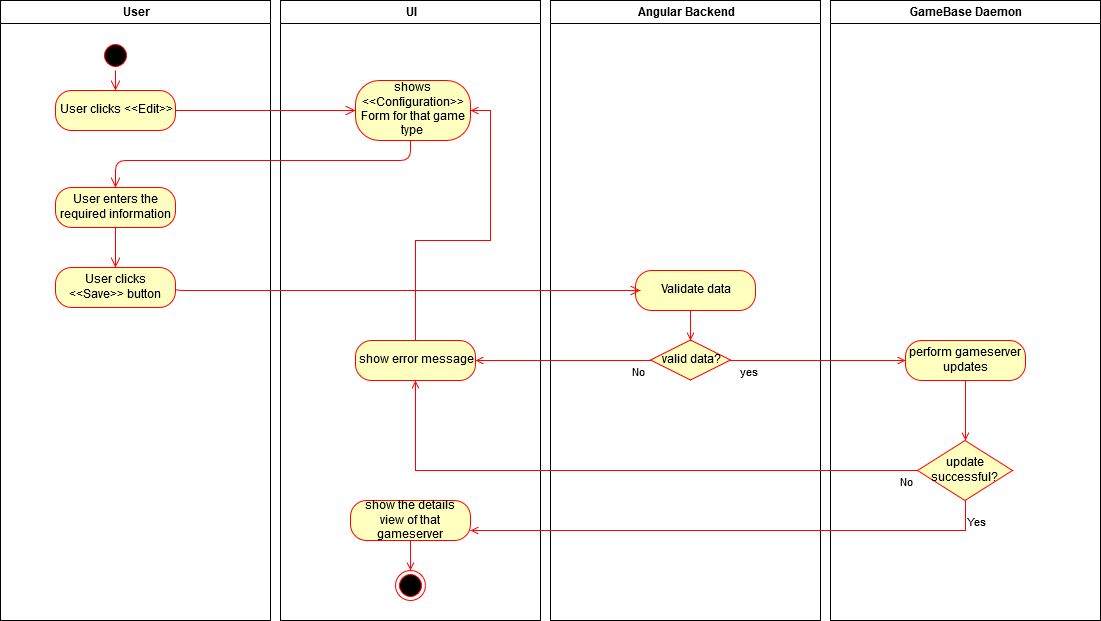
\includegraphics[width=\textwidth]{ConfigureGameserverActivityDiagramm.png}
	\caption{Activity Diagramm}
	\label{fig:ad}
\end{figure}

\section{Basic flow}

\begin{itemize}
    \item User is on a gameservers detail page
    \item User clicks on <<Edit>>
    \item User fills the form with the required information
    \item User clicks on <<Save>> to save the edits and gets redirected to the gameservers detail page
    \item or the User clicks on <<Cancel>> to cancel the update operation and gets redirected to the gameservers detail page
\end{itemize}

\section{Configuration}
[include image]\\
The configuration of an existing gameserver. The user will be asked to input game specific parameters for that gameserver.

\chapter{Special Requirements}

\section{Owning an account}
The user has to be a registered user for our system.

\section{Being allowed to configure that gameserver}
The user needs the permissions to update that gameserver.

\chapter{Preconditions}
\section{Must be logged in}
The user must be logged in to edit a server.

\section{Must be owner or permitted to update the server}
The user must own that gameserver or has the permissions to configure the gameserver, given by the owner of that server.

\section{User navigated on the gameserver details page}
The user must have navigated on the gameservers details page of the gameserver he wants to edit.

\chapter{Postconditions}

\section{Configure}
After configuring a gameserver the user will be redirected to the gamservers details page.

\end{document}